\chapter{One Engine Before Many Buckets}

Grant Mitt's interview is not a blackboard lecture, but it does have a quantitative spine. The numbers are not presented as audited economic data; they are interview claims used to discipline the romance of entrepreneurship. The chapter therefore treats them as source-conscious operating facts: base rates, thresholds, follower counts, percentages, and scaling comparisons that help us ask what kind of risk is actually being taken. The arc is simple and severe: enter the market without hiding behind age, understand the odds, concentrate before diversifying, use media as leverage, learn through sales, scale through people, and protect the energy required to keep operating.

\section{The Market Does Not Care About Age}

The interview begins with a confidence problem. Grant Mitt is young, and the host asks how someone young can operate in an industry where owners and decision makers may be two or three times older. Mitt's answer is deliberately deflationary: if the operator makes age a problem, the market will reflect that hesitation; otherwise the market simply tests performance.

His analogy is the NFL. Once a player is in the league, a rookie and a nineteen-year veteran can both be cut, both can win, and both can compete for the same prize. The business version is that, once we are actively attacking the market, the question is not age but whether customers choose to do business with us.

We can write the operating principle in a compact way. Let \(M\) denote the market's selection mechanism, and let \(a\) be age. Mitt's claim is not that age has no social effect. It is narrower: for the operator's own decision rule, age should not be allowed to become the dominant explanatory variable.

\begin{equation}
  \hbox{Market result} \approx M(\hbox{offer},\hbox{execution},\hbox{trust})
  \quad \hbox{rather than} \quad
  M(a).
\end{equation}

This is not a formal economic model. It is a mental-model correction. If the operator's first explanation for losing is ``I am too young,'' he has already moved attention away from offer, execution, and trust.

\section{Why Start When The Base Rates Are Bad?}

The next question is more serious. The host asks when Mitt decided not to take the corporate route. Mitt answers first with necessity: he had people depending on him, and he felt that he had no choice. But he immediately refuses to romanticize entrepreneurship. In the interview, he says that most people should not simply start a business because the numbers are harsh.

The following claims should be read as Mitt's spoken claims in the interview:

\begin{align}
  \Pr(\hbox{company breaks even or loses money}) &\approx 0.86,\\
  \Pr(R_{\hbox{company}} > \$10{,}000{,}000) &\approx 0.005.
\end{align}

Here \(R_{\hbox{company}}\) denotes company revenue. The second line is the claim that about one half of one percent of companies ever revenue over ten million dollars. The first line is the claim that \(86\%\) of companies in the United States break even or lose money.

Mitt then compares business owners with employees. The transcript gives the rough comparison as ``58 to 55'' and says the employee makes about \(\$3{,}000\) to \(\$4{,}000\) more. The unit is not fully specified, so the safest notation is:

\begin{equation}
  \bar I_{\hbox{employee}}-\bar I_{\hbox{business owner}}
  \approx \$3{,}000 \hbox{ to } \$4{,}000,
\end{equation}

with the verbal caveat that this is an interview claim, not a verified statistic. The point is not precision. The point is that ownership by itself is not a guarantee of wealth.

\subsection{Question \& Answer}

\paragraph{Question.}
Should everyone start a business if they want to build wealth?

\paragraph{Answer.}
No. Mitt's answer is that the choice is not simply employment versus entrepreneurship. A person may be an entrepreneur, but may also be an intrapreneur: someone who builds wealth, responsibility, and upside inside an excellent company. In the interview, he says that people inside Mitt Group can become multimillionaires as intrapreneurs, provided the company gives them room to grow.

The decision tree is therefore not a slogan. It is closer to:

\begin{equation}
  \hbox{Path} \in
  \{\hbox{employee},\hbox{intrapreneur},\hbox{entrepreneur}\}.
\end{equation}

The entrepreneur bears the direct downside. The intrapreneur needs the right firm. The employee may earn more than the average business owner. The serious question is which path gives the person the best combination of capability, upside, and fit.

\begin{table}
\centering
\begin{tabular}{p{0.28\linewidth}p{0.31\linewidth}p{0.31\linewidth}}
\hline
Path & Main advantage & Main condition \\
\hline
Employee & Stable income and role clarity & Limited ownership upside \\
Intrapreneur & Upside inside a strong company & Company must create real room \\
Entrepreneur & Direct ownership and control & Operator bears direct downside \\
\hline
\end{tabular}
\caption{Mitt's distinction between employee, intrapreneur, and entrepreneur, reconstructed from the interview claims.}
\end{table}

Mitt's own reason for starting was that he had to. He says he had the time, resources, capital, and preparation, and he was willing to lose every penny knowing that he had tried. That is a very different claim from ``business is automatically better than a job.''

\section{Concentration Before Diversification}

The next major pivot is the diversification question. The host asks how important it is for entrepreneurs to diversify beyond one or two hustles. Mitt's answer is blunt: he does not think people should diversify early. He invokes the familiar claim that the average millionaire has seven income streams, but then reverses the usual lesson. In his telling, the seven streams usually come after one thing made the person wealthy.

The operating threshold in the interview is:

\begin{equation}
  R_{\hbox{solar}} > \$10{,}000{,}000
  \quad \Longrightarrow \quad
  \hbox{begin considering diversification}.
\end{equation}

This is a threshold, not a universal law. It is Mitt's account of his own sequence: he did not start diversifying until the solar company was over ten million dollars in revenue. Even then, he says most of his focus and energy remained on solar.

The mechanism is worth preserving. First make the big pile. Then allocate from it into buckets that can produce additional cash flow. If there is no big pile, diversification often means being mediocre at several things rather than excellent at one.

\begin{figure}
\centering
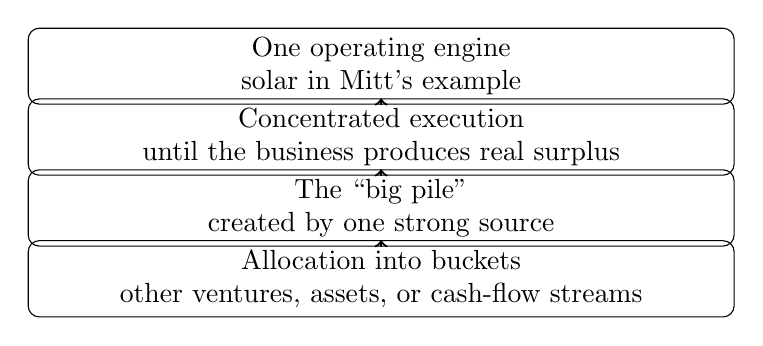
\begin{tikzpicture}[
  node distance=0.9cm,
  box/.style={draw, rounded corners, align=center, text width=0.72\linewidth, minimum height=0.9cm},
  arrow/.style={->, thick}
]
\node[box] (engine) {One operating engine\\solar in Mitt's example};
\node[box, below of=engine] (mastery) {Concentrated execution\\until the business produces real surplus};
\node[box, below of=mastery] (pile) {The ``big pile''\\created by one strong source};
\node[box, below of=pile] (buckets) {Allocation into buckets\\other ventures, assets, or cash-flow streams};
\draw[arrow] (engine) -- (mastery);
\draw[arrow] (mastery) -- (pile);
\draw[arrow] (pile) -- (buckets);
\end{tikzpicture}
\caption{The interview's concentration-before-diversification logic. The diagram is a reconstruction from the transcript, not a screenshot-backed board figure.}
\end{figure}

The transcript also contains projected revenue language: Mitt says the solar company will ``revenue 30 this year'' and then ``90, 120'' next year. The units are not explicitly stated in that sentence, though the surrounding context suggests millions of dollars. A cautious notation is:

\begin{equation}
  R_{\hbox{solar,this year}} \approx 30,
  \qquad
  R_{\hbox{solar,next year}} \approx 90\hbox{ to }120,
\end{equation}

where the likely unit is millions of dollars, but the chapter should not overstate what the transcript does not explicitly say.

\section{Media As Leverage Around The Main Business}

Only after the concentration argument does the interview turn to content. This order matters. Social media is not presented as a substitute for the operating business. It is presented as leverage around it: credibility, recruiting, connection, and brand.

The host notes that Mitt has built a following of over \(100{,}000\) people. Mitt gives more specific numbers:

\begin{equation}
  F_{\hbox{TikTok}} \approx 145{,}000,
  \qquad
  F_{\hbox{Instagram}} \approx 25{,}000.
\end{equation}

He also gives a recruiting anecdote. In a company-wide meeting, among six or seven new starters, he says that \(30\%\) to \(40\%\) reported that they had been following him or found the company through social media.

\begin{equation}
  \Pr(\hbox{new starter linked to Grant's social presence})
  \approx 0.30 \hbox{ to } 0.40.
\end{equation}

This is a good example of a non-direct sales channel. Content does not merely sell a product; it changes who hears about the company, who trusts it, and who is willing to work there. Mitt says that Fox Business appearances and other media opportunities would not have happened simply because the company was larger. They happened because he had a visible individual brand.

The principle can be stated as:

\begin{equation}
  \hbox{Media leverage}
  =
  \hbox{trust}+\hbox{reach}+\hbox{recruiting surface},
\end{equation}

again as a schematic, not a formal identity. The transcript's point is practical: free information and public presence can create opportunities that the operating company alone may not create.

\section{Risk, Sales, And Learned Confidence}

The risk section begins with a large claim: risk-taking is everything. Mitt immediately qualifies it. There are times to be risk-on and risk-off; one must prepare for a rainy day; one has to be smart. The deeper claim is that risk becomes rational when it is backed by ability.

Mitt's vivid image is that he does not want to wait until age seventy-five to enjoy the rewards of risk. He wants the optionality earlier, when it can affect life, family, and the ability to help people. Then he adds the Sahara Desert image: if he lost everything but kept his mind and ability intact, he believes he could rebuild faster because he now knows how the game works.

A careful reconstruction is:

\begin{equation}
  \hbox{Willingness to risk}
  \uparrow
  \quad \hbox{as} \quad
  \hbox{earned capability and self-trust} \uparrow.
\end{equation}

The self-trust is not mystical. Mitt defines it through kept promises and performance under pressure. We can write the update rule in a deliberately simple form. Let \(C_t\) be confidence at time \(t\), not as a feeling but as an estimate of one's own ability to execute. After a hard commitment, confidence updates according to whether the operator performs.

\begin{equation}
  C_{t+1}
  =
  C_t
  +
  \alpha(\hbox{promise kept})
  -
  \beta(\hbox{promise broken}),
  \qquad
  \alpha,\beta>0.
\end{equation}

This is not in the transcript as an equation. It is a note-writing reconstruction of Mitt's mechanism: confidence increases when promises to oneself are kept, and risk becomes easier when the operator has evidence that he executes under stress.

\subsection{Question \& Answer}

\paragraph{Question.}
Why can't sales skill be learned from a textbook?

\paragraph{Answer.}
Because the skill being described is not merely verbal technique. Mitt says, ``You can't Google experience.'' The sales lesson comes from repeated contact with rejection: cold calls, doors, being told no, being cursed out, and still delivering the message correctly.

A compact way to write the learning process is:

\begin{align}
  \hbox{attempt}_{t} &\longrightarrow \hbox{customer response}_{t},\\
  \hbox{customer response}_{t} &\longrightarrow \hbox{adjusted message}_{t+1},\\
  \hbox{many repetitions} &\longrightarrow \hbox{judgment}.
\end{align}

This is the sales version of empirical learning. The operator learns what works and what fails across ages, backgrounds, temperaments, and situations. Mitt's example is selling DirecTV inside Walmart at ages eighteen or nineteen, when customers were buying groceries, tired from work, or simply uninterested. That difficulty is the curriculum.

\section{Scaling Means People, Not Gadgets}

The scaling section begins with a concrete count. The host asks how many states Mitt Group is closing solar deals in, and Mitt answers:

\begin{equation}
  N_{\hbox{states}} = 17.
\end{equation}

From there, the question becomes how a company moves from six or seven figures to eight figures. Mitt's definition is short: scaling is doing the little things right at scale. The warning is that people try to expand before they have conquered the current place. They ask whether to go to Europe or another city before they are crushing the present market.

The quantitative contrast is important. Mitt says that a CRM, a cool technology, or hiring one smart person might help by \(10\%\) or \(20\%\), but it will not double, triple, or quadruple revenue by itself.

\begin{equation}
  \Delta_{\hbox{tool/CRM/smart hire}}
  \approx 10\%\hbox{ to }20\%,
  \qquad
  \Delta_{\hbox{true scale}}
  \in \{2\times,3\times,4\times,\ldots\}.
\end{equation}

So the mechanism of scale is people. A billion-dollar company requires thousands of people who know what they are doing, including people as smart or smarter than the founder in specific areas. The founder cannot be overshadowing every action.

\paragraph{Worked scaling example.}
Suppose a business has revenue \(R_0\). A tool improvement of \(20\%\) gives

\begin{equation}
  R_1 = 1.20R_0.
\end{equation}

That is useful, but it is not the same as tripling:

\begin{equation}
  3R_0 - 1.20R_0 = 1.80R_0.
\end{equation}

The missing \(1.80R_0\) cannot be explained by the tool alone in Mitt's account. It has to come from repeatable execution by trained people, operating without the founder doing everything for them.

\begin{table}
\centering
\begin{tabular}{p{0.30\linewidth}p{0.30\linewidth}p{0.30\linewidth}}
\hline
Scaling input & Transcript claim & Mechanism \\
\hline
CRM or technology & May add \(10\%\) to \(20\%\) & Improves process efficiency \\
One smart hire & Helpful but insufficient alone & Adds local capability \\
Many trained people & Required for real scale & Distributes execution \\
Founder oversight & Cannot be everywhere & Must be replaced by systems \\
\hline
\end{tabular}
\caption{Mitt's distinction between incremental improvement and true scale.}
\end{table}

The chapter should preserve the force of this section. Scaling is not presented as a software purchase or a clever hack. It is the multiplication of fundamentals through people.

\section{Energy, Industry Choice, And The Hiring Filter}

The final movement turns inward again. The host asks how Mitt avoids burnout. Mitt's answer is another resource model: each person wakes up with a certain amount of energy, and every communication, interaction, and decision drains some of it. Therefore the word ``no'' becomes important.

Let \(E_t\) denote available energy during a day. If each interaction \(i\) consumes \(c_i\), then a simple bookkeeping model is:

\begin{equation}
  E_{\hbox{remaining}}
  =
  E_0 - \sum_i c_i.
\end{equation}

The point is not physiology. The point is managerial selectivity. If an appointment goes badly and the operator spends emotional energy being angry, that cost is carried into the next appointment. Burnout, in Mitt's account, comes from poor control of energy and emotion, not simply from working hard.

He then adds three stabilizers:

\begin{itemize}
  \item stay level-headed through highs and lows;
  \item manage energy and emotional response;
  \item use plans, processes, and systems so winning becomes repeatable.
\end{itemize}

The industry-choice question comes next. Mitt says that in the 2014--2016 period he looked for industries likely to be bigger in twenty years than they were then: technology, AI, robotics, renewable energy, and crypto. He did not claim to know all of them deeply at the start. He looked for a place where he could get a foot in the door and learn.

This is a market-selection rule:

\begin{equation}
  \hbox{Good arena}
  =
  \hbox{future growth}
  +
  \hbox{room to enter}
  +
  \hbox{chance to learn}.
\end{equation}

The final hiring answer closes the loop. Mitt says the non-negotiables are coachability, humility, and persistence. He does not care how talented someone was elsewhere if that person cannot be coached. He also makes a hard claim about necessity: people with a comfortable fallback often do not push through; people who have to make it find a way.

The hiring filter can be summarized as:

\begin{equation}
  \hbox{Hire}
  \Longleftarrow
  \hbox{coachable}
  \wedge
  \hbox{humble}
  \wedge
  \hbox{persistent}
  \wedge
  \hbox{no easy fallback}.
\end{equation}

As before, this is a reconstruction of the operating logic, not a board equation. It keeps the structure of the interview: market selection chooses the arena; hiring chooses the people who can survive inside it.

\section{Summary}

This interview gives us an entrepreneurship chapter built around disciplined selection. First, the operator must stop treating age as the decisive variable and let the market test the offer. Second, starting a company must be judged against base rates, not ego; entrepreneurship, intrapreneurship, and employment are distinct paths. Third, diversification comes after concentrated strength, not before it. Fourth, media can compound credibility and recruiting, but it does not replace the main business. Fifth, risk becomes rational when it is backed by skill earned through hard repetitions, especially sales. Finally, scale requires people, energy control, industry judgment, and a hiring filter severe enough to protect the operating system.